Android was designed to protect applications considering both security-oriented developers and those less familiar with safety concerns. By default, Android enforces good levels of protection, inheriting the Linux security model, but also applying its own mechanisms. It is provided with a multi-layered security that supplies the flexibility required for an open platform, while providing protection for all users of the platform \cite{SecurityOverview:Android}. This chapter introduces a general overview into Android security features.

\section{System and Kernel Level Security}

The Android platform comprises three main blocks: device hardware, operating system and application runtime. Each block presents secure mechanisms that are briefly described in the following sections. 

\subsection{Linux Security}

Android has inherited security mechanisms from the Linux kernel, namely, a user-based permissions model, process isolation and extensible mechanism for secure \gls{ipc}. The user-based permissions model was originally developed for Unix environments, thus Linux takes advantage of it. In fact, the user-based permissions model has proven its good design concerning security issues over time. Every user registered in the system has an unique identifier number known as \gls{uid}. Along with users, there are groups that are identified by its unique \gls{gid}. One group might have one or more users, and one user might belong to one or more groups. Note that all users belong to at least one group, which is the group that contains all users. Every resource in the system, or in simple terms, every file in the system has an owner, that is identified by its \gls{uid}. This owner has the responsibility over the file and is able to alter its permissions. Files have also a group associated which is identified by its \gls{gid}. Each file on a Linux system has three sets of permissions: owner, group and world. The owner and the group are those mentioned before. The world is considered to be every user registered on the system. Each file might be accessed by three types: read, write and execute. So, each set of permissions can include read (r), which allows an entity to read the file; write (w) which allows an entity to write the file; and execute (x) which allows an entity to execute the file. According to its permissions, a file may be read and/or wrote and/or executed by its owner, that has an unique \gls{uid}, and/or by every member of the file's group, and/or by all other users that have an account on the system \cite{ComputerSecurity}.

\subsection{Application Sandbox}

Using the user-based permissions model, the system's resources have a robust access control. Android took this feature and built an application sandbox where each application can only access its own files and components (unless the developer grants other permissions that we'll see later). When an application is installed on the system, an new unique \gls{uid} is assigned to it and the application runs under this \gls{uid}. In addiction, all data stored by that application is assigned the same \gls{uid}. The Linux permissions are set on this application to allow read, write and execute access by its owner and no permissions otherwise. This mechanism is illustrated in \autoref{fig:android_sandboxing} \cite{AndroidSecurityUnderpinnings}.

\begin{figure}[h]
 \begin{center}
 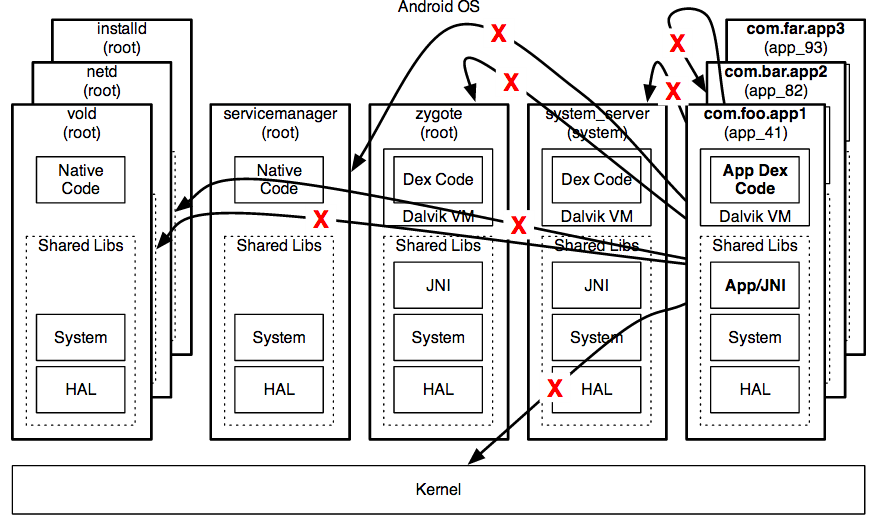
\includegraphics[scale=0.5]{figures/android_security.png}
 \end{center}
 \caption{Application sandboxing}
 \label{fig:android_sandboxing}
\end{figure}

\subsection{Filesystem Isolation}

The user-based permissions model is also used to provide filesystem isolation, which fits in the application sandboxing model. Android creates a specific directory to each installed application under the path \texttt{/data/data/}. Each directory is configured such that the associated application's \gls{uid} is the owner and only its permissions are set. Within this directory is \texttt{/files} directory that stores all files created by the application. These files are granted the same permissions and run under the owner's \gls{uid}, providing isolation access from other applications. This access control is enforced to all applications. However, if a user access the Linux kernel using the root \gls{uid} will break down the sandboxing mechanism and be able to access any data stored in any application.

Linux permissions access control works on every Android filesystem except on the SD card (\texttt{/sdcard} directory). Therefore, any file written to external storage is accessible by any application.

\subsection{Security-Enhanced Android}

As mentioned above, the user-based permissions model grants protection from the Android foundations. However this model enforces a \gls{dac} mechanism that increases the risk of harm, as we will see later in the \gls{lsm} section. To overcome the related threats, Android began to use a component that has been in the Linux kernel in the last years, \gls{sel}. This mechanism applies a \gls{mac} model \cite{SEAndroid} that reduces the effect of malicious software and protect users from potential flaws in code \cite{SELinux:Android}. 

\section{Android Application Security}

Android applications extend the core Android operating system. The previous security features were not able to ensure the protection level desired to a world wide used mobile platform as Android, therefore a set of artifacts were developed granting applications safety in a satisfactory degree. They are briefly described as follows.

\subsection{Manifest Permissions}

Besides the user-based permissions model adopted from the Linux kernel, Android brought a new permissions model know as \textit{Manifest permissions}. As mentioned earlier, each application is only allowed to access its own data, by default. However, Android offers a lot of resources and libraries so that developers can build powerful and useful applications. But, the gain of power brings security vulnerabilities. For instance, Android provides network resources that allow applications to establish internet communications. But, malicious applications could take advantage of this feature and use it to spread user's personal data.


Google decided to implement the Manifest permissions model that forces developers to specify which resources their applications use when executing. Each resource requires a permission that must be declared on the Manifest file. At installation time, permissions are set to the application and it will only have access to the declared resources. Using the previous example, if the developer wants to use network resources, he declares the INTERNET permission through the following statement:

\noindent \texttt{<uses-permission android:name="android.permission.INTERNET"/>}

\noindent on the Manifest file. Before the installation, the user gets the list of all Manifest permissions. This feature brings two main advantages. First, it alerts the user to all possible dangerous actions the application may take. For instance, if the user intends to install a simple game and the Manifest file exhibits SMS and phone call permissions, which means that the application can send SMS and make phone calls, something doesn't seem to be right. The user makes his judgement and decides to either install or not install the application. The second advantage ensures the protection of the application against malware. In the case of one application gets compromised, the attacker will only be able to access the resources that the application was allowed to. For instance, if an application that takes photos has only permission to use the camera and gets compromised, the attacker will only be able to access the camera and none of the remaining resources that need Manifest permission.


Android comprises a large set of Manifest permissions \cite{ManifestPermissions:Android} and regular applications take advantage of a considerable amount of them. Since there is a considerable set of permissions that causes no harm to the device, users don't need explicitly to accept them in order to install applications. Therefore, Google established four categories where Manifest permissions falls into, described as follows:

\begin{itemize}
 \item \textbf{Normal}. Permissions to access inoffensive resource. For that reason they are granted by default. As example, the permission to change the device's background;

 \item \textbf{Dangerous} Permissions to access resources that might cause harm to users. In this case, users must accept them before the installation. As example, the permission to access 
private data, or establish internet connections;

\item \textbf{Signature} Permissions that were required by other applications signed with the same digital certificate. If the application is signed by the same certificate as the declaring app, the permission will be granted; if not, the app being installed will no be granted the permission. The user is never questioned about these permissions in order to start an installation;

\item \textbf{SignatureOrSystem} These permissions follows the same rule as \textit{Signature} permissions, but adding a new rule that checks the Android system image. This type of permission is used by device manufacturers to allow applications created by different vendors to work together within that Android builds.
\end{itemize}


An important rule that follows the Manifest permission is the Principle of Least Privilege \cite{ApplicationSecurity:Oreilly}, which states that each application should keep permissions at its minimum, using the weak permission instead of a strong one that allows the application to execute tasks that will not be called. For instance, if the application only needs to read contacts, the permission required should be \texttt{READ\_CONTACTS} and not full access to contacts that also allow to write contacts.

\subsection{Application Signing}

Google requires all Android applications to be signed through a digital certificate, being the private key held by the application's developer. This process ensures the authentication of a developer when he's trying to deploy his application into the market and establishes trust relationships between applications. Signing an application does not require a \gls{ca}. In fact, most of Android applications are self-signed by developers. Google released tools that allow developers to sign their applications and provides useful documentation to facilitate the process \cite{AndroidSigning:Android}.


The Application signing process concede an useful feature to developers that build more than one application. As mentioned earlier, each application is assigned an unique \gls{uid} and is not allowed, by default, to share data and resources with other applications. However, if an user installs more than one application signed by the same developer, which means the same digital certificate, and these applications declare the \texttt{shareUserId} attribute in the Manifest file, Android assigns these applications the same \gls{uid}. Therefore, they are seen by the Linux kernel as the same application and are able to share data and resources.

\subsection{Android Security Overview by Google}

Android Security chief, Adrian Ludwing, presented the Google's approach to fight malware and statistical data regarding infected devices \cite{VBAndroidPracticalSecurity} . Android enforces several layers of protection since the user accesses Google Play until the application is running on its device. These layers were introduced as follows:

\begin{itemize}
\item Google Play;
\item Unknown Sources Warning;
\item Install Confirmation;
\item Verify Apps Consent;
\item Verify Apps Warning;
\item Runtime Security Checks;
\item Sandbox and Permissions.
\end{itemize}

Google Play requires developer information and application signing. Furthermore, each application is reviewed before it becomes available. This process involves a set of procedures that checks static code dynamic behaviors. Heuristics and similarities on-device data are applied. After the analysis it is assigned a probability of threat tag to the application, being \textit{Block}, \textit{Warn} or \textit{Allow}.

Android does not allow the installation of applications from unknown sources by default. This feature ensures that all installed applications had passed the Play Store test. If the user disables this rule by allowing unknown sources, the following alert is displayed \textit{"Your phone and personal data are more vulnerable to attack by apps from unkown sources. You agree that your are solely responsible for any damage to your phone or loss of data that may result from using these apps"}. Also, the feature \textit{Verify Apps} inspects applications prior to install, applying an additional layer of security. If the application presents suspicious code, the installation process might be blocked, in sever cases, or triggers a warning. This is quite useful for those applications that skip the Google Play process review, i.e. were installed from third-party sources.
